\chapter{Feasibility Document Generation}

\section{Introduction}

The Feasibility PPP Document Generation tool revolutionizes the reporting and analysis process in Public-Private Partnerships by automating the extraction of data from Excel files and generating comprehensive reports. This innovative tool leverages artificial intelligence to transform quantitative data into descriptive narratives, significantly enhancing the efficiency and depth of PPP scenario assessments. Designed to streamline the creation of reports and improve decision making, it represents a pivotal advancement in leveraging technology for PPP project management. This chapter outlines the development, functionalities, and impact of the tool on simplifying complex data analysis within the PPP framework.

\section{Objectives}

The AI-powered PPP document generation tool is designed with strategic objectives to enhance Public-Private Partnership project management and reporting. By automating data extraction and analysis from Excel files through artificial intelligence, it transforms complex quantitative information into accessible, descriptive narratives. This key feature streamlines the creation of detailed reports, improving their quality by offering deep insights into the data, thus aiding in clearer understanding and decision-making.
\vskip 0.5cm
Efficiency is a central objective, with the tool reducing manual effort and time traditionally required in the compilation of reports. It frees stakeholders to focus on the strategic aspects of project management. Design also supports informed decision-making by providing comprehensive but straightforward reports that highlight essential data insights, guiding stakeholders toward well-informed decisions.
\vskip 0.5cm
Scalability and adaptability are intrinsic to the tool, designed to meet the varied demands of different PPP projects and sectors. This flexibility ensures that it can be a valuable resource in diverse scenarios, enhancing its utility and application.
\vskip 0.5cm
The anticipated outcomes include increased report accuracy, efficiency in resource allocation, improved stakeholder engagement through clearer communication, and the provision of data-driven insights for better risk management and opportunity identification. Adopting this advanced technology also enhances an organization's competitive edge, showcasing a commitment to innovation and operational efficiency in PPP projects.
\vskip 0.5cm
In summary, this tool represents a significant step forward in leveraging technology to streamline PPP project evaluations, promising a combination of improved efficiency, accuracy, and strategic insight.

\section{Document Generation Architecture}
The system architecture of the AI-powered PPP Document Generation tool encapsulates a highly coordinated process that transitions data from initial input to final output. This process is delineated in the following components as shows the \textbf{Figure \ref{fig:reportGen}}:
\begin{figure}[H]
    \label{fig:reportGen}
    \centering
    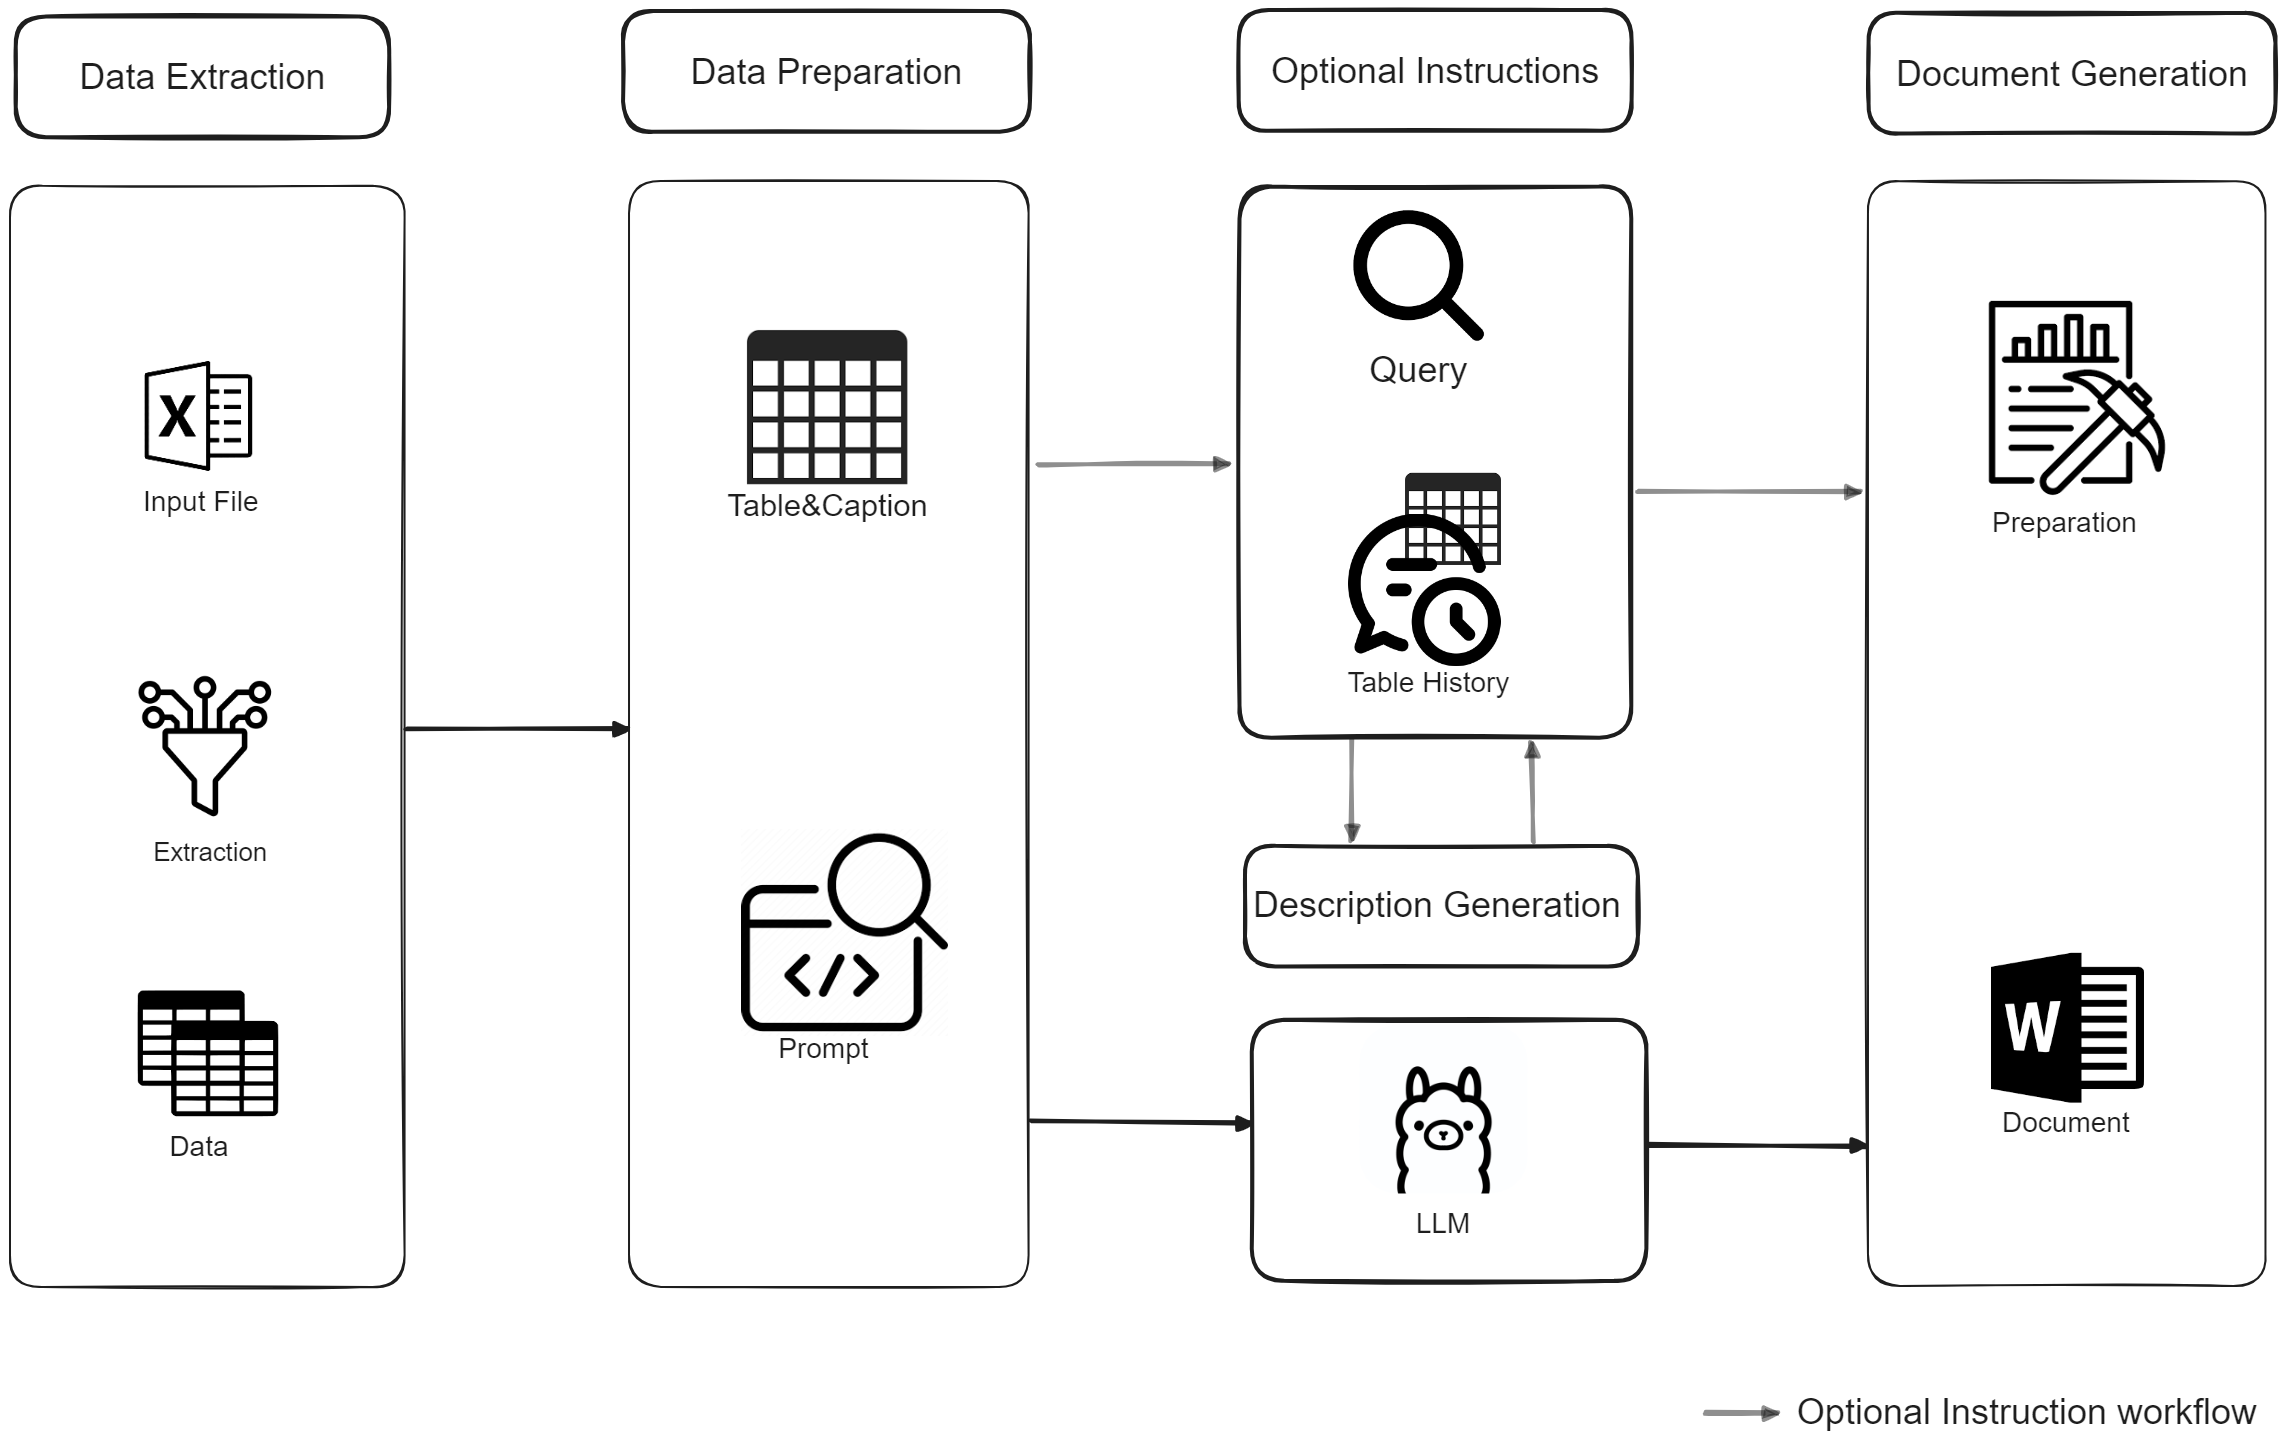
\includegraphics[width=1 \linewidth]{assets/docGenfin.png}
    \caption{Document Generation Architecture }
\end{figure}
The workflow starts with the Data Extraction phase , a significant beginning point where raw information is gathered from an Excel file . This stage is foundational, focusing on identifying and gathering titles, tables, and the captions that illustrate the context of each table. Extraction tools are deployed to automate this process , guaranteeing that the data is pulled accurately and efficiently . The result are a compilation of natural data , which is an accumulation of figures, content , and names ready for the another stage of refinement.
\vskip 0.5cm
Following extraction, the Data Preparation phase commences. Here, the raw data experiences a transformation into a structured format conducive to examination . This includes sorting, cleaning, and organizing the data into coherent tables accompanied by descriptive captions. In pair , a well-crafted prompt functions as a directive for the consequent analytical process . The prompt encapsulates specific instructions and objectives that guide the dealing with and interpretation of the information , setting the stage for the application of advanced analytical procedures .
\vskip 0.5cm
Consolidating a layer of adaptability into the workflow are the Optional Instructions . This intermediary step isn't always actuated but serves as significant part when utilized. It permits for the integration of custom queries and extra orders that relate to the historical perspectives of the information or particular analytical requirements . This flexible component guarantees that the following examination isn't as it were strong but too custom fitted to the interesting necessities of the project or the questions at hand.
\vskip 0.5cm
With the information prepared and prompts in place , the Description Generation phase leverages the capabilities of a Large Language Model (LLM ). The AI ingests baseline data from the prepared information , if provided , to synthesize a description. This story may be a nitty gritty , AI generated composition that dives into the insights inferred from the information. It contextualizes numbers and patterns inside the tables, weaving them into a description that's both informative and available to the intended audience.
\vskip 0.5cm
The perfection of the workflow is the Document Generation phase . The wealthy , descriptive content delivered by the LLM is  fastidiously gathered into a formal report , typically a Word file . This document encapsulates the analytical journey from raw data to Description, insights and presents it in an format that's cleaned and prepared for spread . The document not only describes the findings but is also structured in a way that coordinating visual components , such as merging cells and styling, which improve comprehension and give a visual outline of the literary investigation .
\vskip 0.5cm
Additionnaly, these stages represent a spic-and-span and modern prepare , changing tables from an Excel spreadsheet into a narratively wealthy and visually supported document that is both comprehensive and prepared for professional PPP report.
% \begin{itemize}
%     \item \textbf{Data Extraction:} The initial stage involves extracting quantitative assessment data from Excel files. This data is critical for generating the PPP reports and represents the raw input for the system.
    
%     \item \textbf{Dataframe and Dictionary Conversion:} Post-extraction, the data is not transformed into JSON but is instead loaded into a pandas DataFrame within a Python dictionary. This structure is highly efficient for handling tabular data and supports a wide array of operations required for subsequent processing stages.
    
%     \item \textbf{Array Transformation:} Before the data is input into the AI model, the pandas DataFrames, encapsulated within Python dictionaries, are transformed into arrays. This step is essential for compatibility with the LLM, ensuring that the data is in a suitable format for narrative generation.
    
%     \item \textbf{Custom Prompt and Description Generation:} Armed with the structured array, a custom prompt template — enhanced with the table data — is created. This custom prompt, in conjunction with the array, is fed into a Large Language Model (LLM) which is then tasked with generating a descriptive paragraph that provides qualitative insights derived from the quantitative data.
    
%     \item \textbf{Document Templating:} Simultaneously, a document template is devised, which defines the desired layout and formatting of the final document. This template ensures consistency and adherence to reporting standards.
    
%     \item \textbf{Document Generation:} At the heart of the system is the document generator component, which synthesizes the descriptive narratives from the LLM with the array-based data and merges them into the predefined document template. This process culminates in the creation of a comprehensive and formatted document.
    
%     \item \textbf{Output Document Formats:} The output is then furnished in a choice of formats, such as DOCX for editable documents or PDF for fixed layout presentations, accommodating diverse dissemination requirements.
% \end{itemize}
% This architecture acknowledges the specific data structures employed and the precise transformation steps taken, ensuring a clear and accurate representation of the tool’s functional design.

\section{Data Extraction}

\subsection{Input File}
The foundation of our data-driven approach starts with the Input File , typically an Excel file \textbf{Figure \ref{fig:excl}}, containing different spreadsheet, each one includes sheet title, tables, and corresponding captions. These records represent the raw material from which valuable insights are to be extracted and afterward refined into a comprehensive report.

\begin{figure}[H]
    \centering
    
\includegraphics[width=0.5 \linewidth]{assets/excel.png}
    \caption{Input File}
    \label{fig:excl}
\end{figure}

\subsubsection{spreadsheet sample}
The spreadsheet, as demonstrated on \textbf{Figure \ref{fig:dataset}} is a collection of tables, each with a unique title wich is the title of the sheet and a caption that gives insights for the data. Besides, The expressive caption of ceratin table clarifies the content and significance of the table itself. However, The tables contain quantitative data that's fundamental for creating the PPP reports. The dataset is structured in a tabular format , with rows and columns representing the data points and categories, respectively . This structured dataset serves as the essential input for the AI powered report generation tool , empowering the extraction of valuable insights and the creation of detailed reports.
\begin{figure}[H]
    \centering
    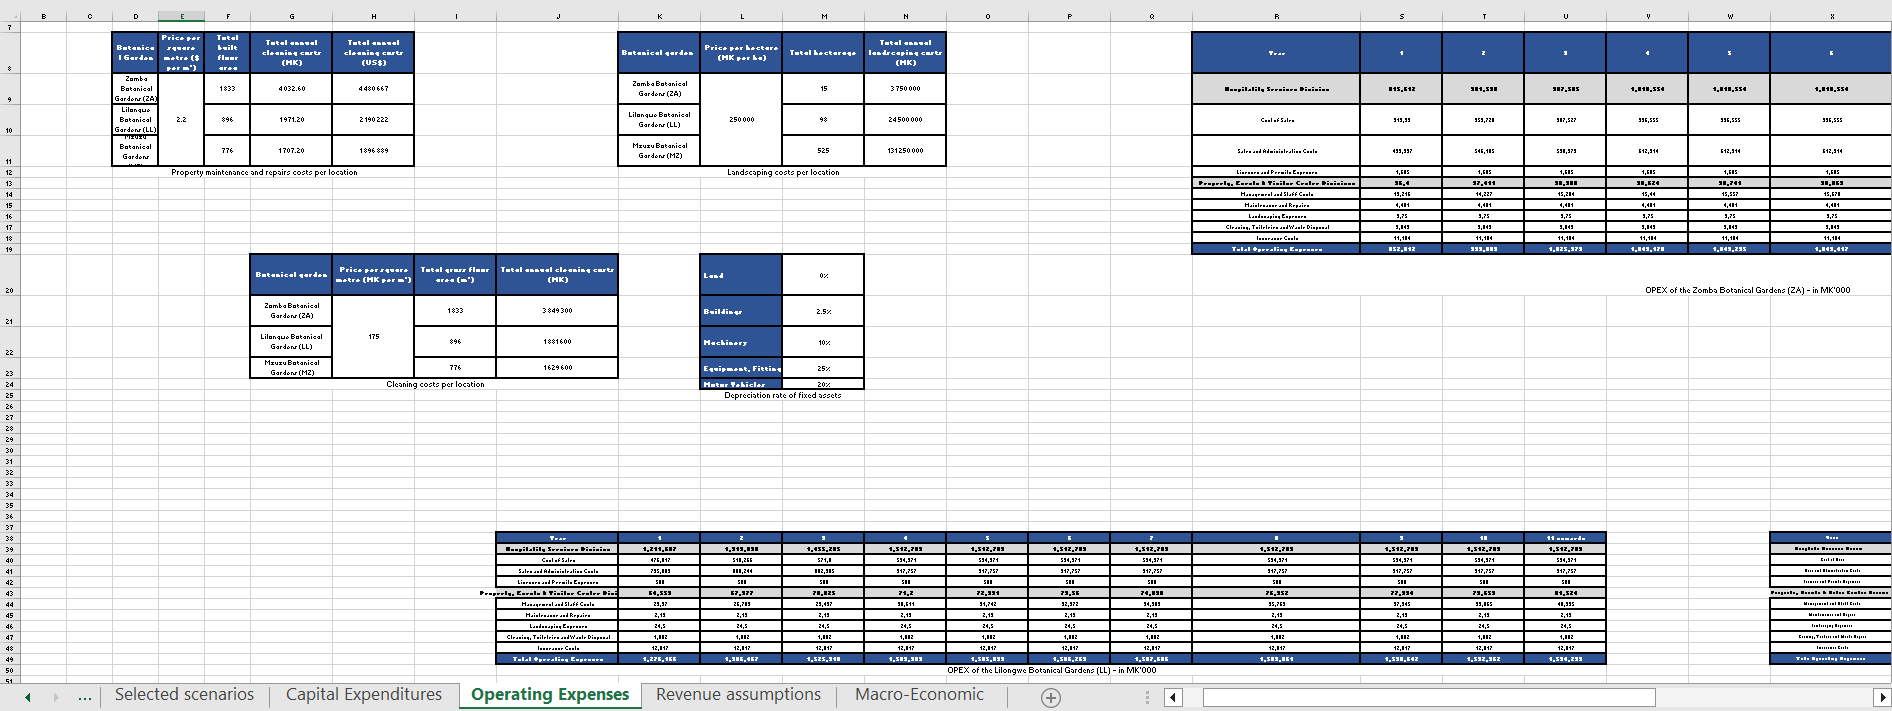
\includegraphics[width=1 \linewidth]{assets/dataExcel.png}
    \caption{Sample of dataset}
    \label{fig:dataset}
\end{figure}
Obviously, When working with spreadsheets, it's easy to get lost in all the numbers and information. But there are some simple things we can do to make them easier to follow:

\begin{itemize}
    \item \textbf{Don't Make Cells Too Complicated:} Sometimes, we might think it looks better to combine cells together, but it actually makes things harder to read. Instead of merging cells, just repeat the data in each cell. This way, everything remains clear and organized.
    
    \item \textbf{Fill in Empty cells:} If there are empty spaces in your spreadsheet, it can be confusing. To settle this, just put a dash '-' in those spaces. This indicates that there's no data there, so no one gets confused.
    
    \item \textbf{Make Titles and Captions Unique:} It's imperative to provide each part of your spreadsheet a different title. If you use the same title or caption more than once, it can be confusing. So, always make sure each title or caption is different from the others.
    
    \item \textbf{Keep Tables Separate:} Sometimes spreadsheets can get really enormous and untidy, with lots of different tables mixed together. This may make it difficult to understand what's going on. Attempt to keep each table on its own sheet, so it's easier to see what belongs together.
\end{itemize}

By following these simple tips, we could make our spreadsheets much easier for the extraction process.
\subsection{Data Extraction Process}

In this stage, the essential tool utilized for extracting tables from Excel files is eparse library, a robust library designed particularly for recognizing and parsing organized data inside spreadsheets. This tool proficiently handles the extraction of numerous tables from a single Excel file , recognizing particular table structures through their layout. Upon loading an Excel file into the system , eparse analyzes the spreadsheet to identify delineations between distinctive data squares , recognizing empty cells, corners, and the boundaries of each table. It can recognize tables that are closely positioned however separate , and indeed perceive subtables inside bigger tables based on varieties in organizing or column arrangements . This capability permits us to efficiently extricate each table as a discrete dataset.

\begin{figure}[H]
    \centering
    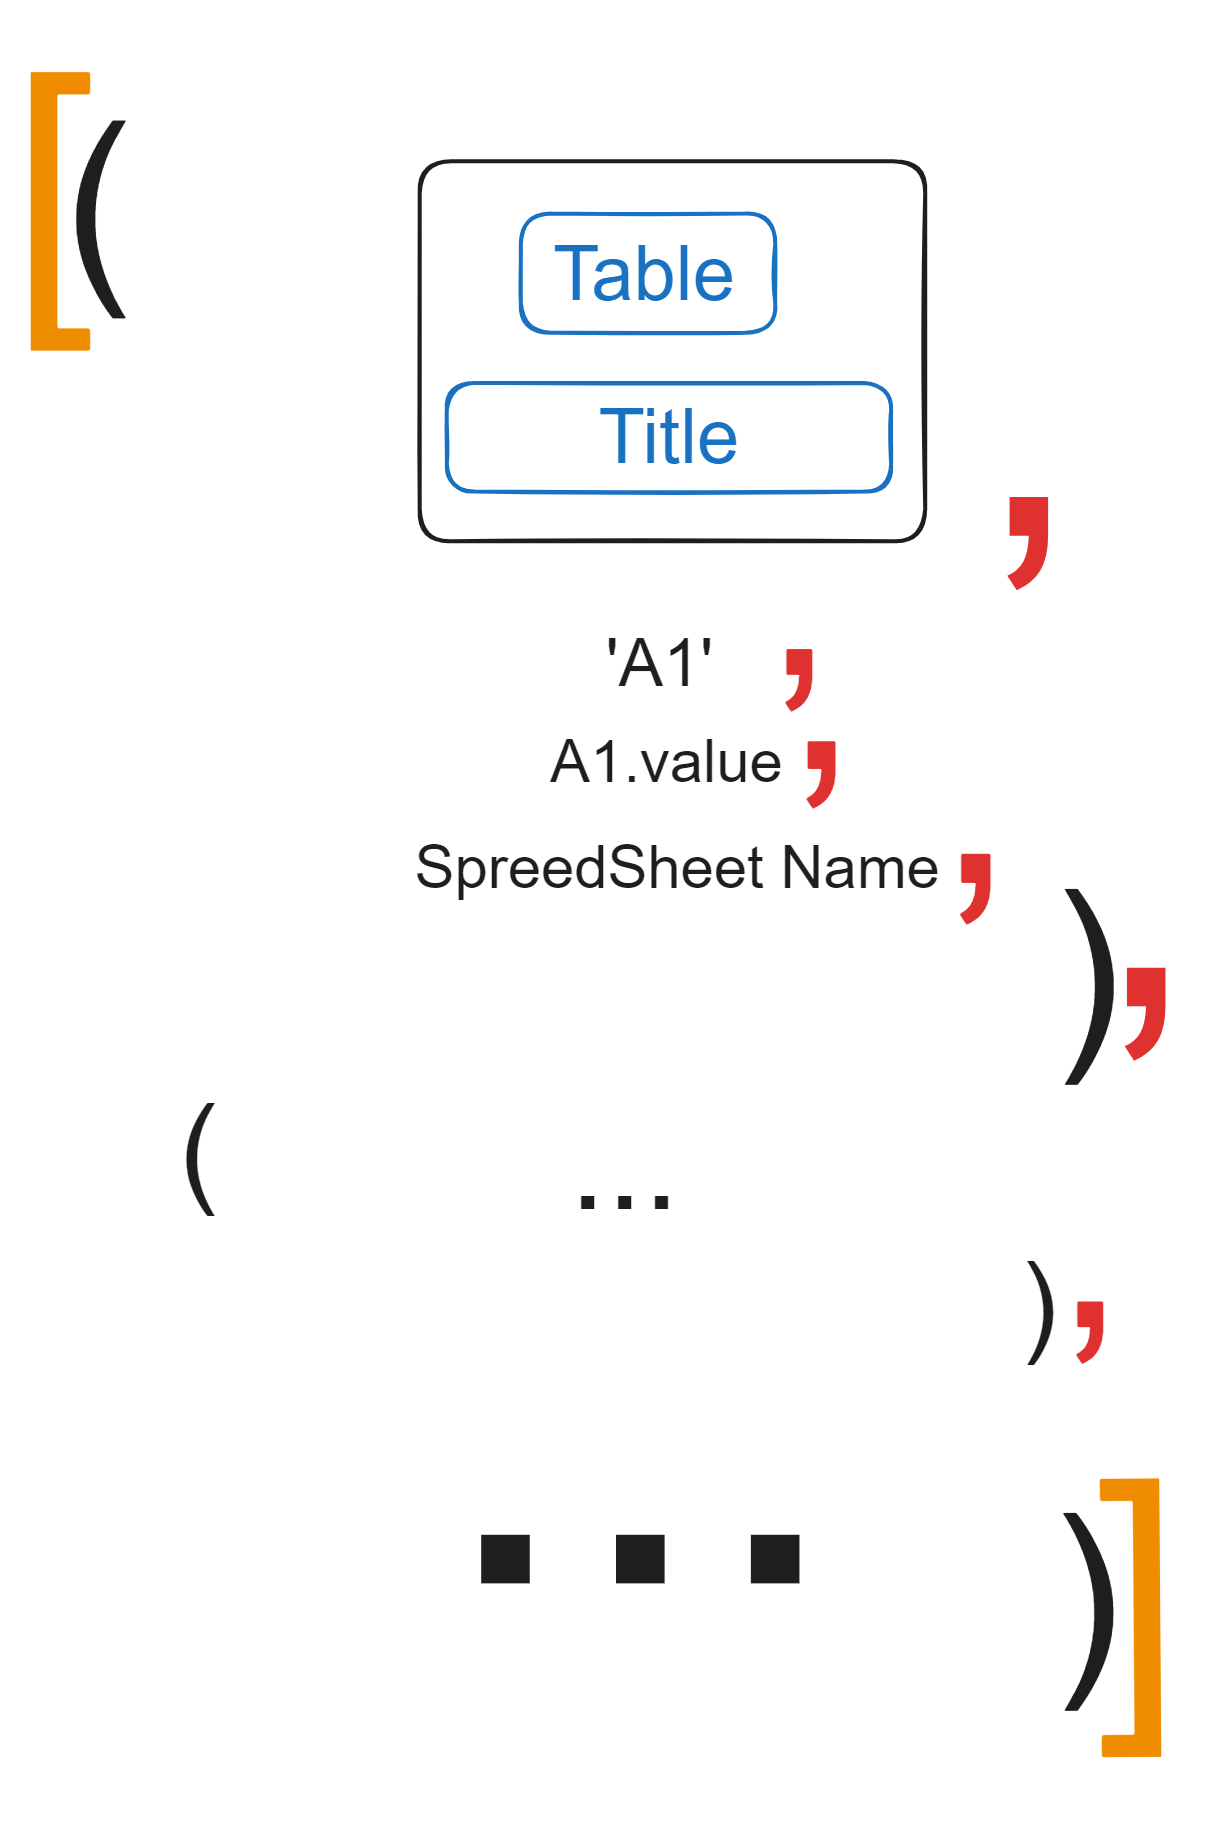
\includegraphics[width=0.4 \linewidth]{assets/eparse_output1.png}
    \caption{Extracted Data Structure}
    \label{fig:extstruct}
\end{figure}

the accompanying \textbf{Figure \ref{fig:extstruct}} serves as a visual abstraction of the eparse tool's functionality in extracting table data from an Excel spreadsheet. Central to the figure may be a representation of a spreadsheet table, indicated by the names Table and Title, demonstrating the distinguished table and its corresponding title. Flanking the table are curly braces, which, in programming contexts , typically encapsulate a related set of information or a code block . This suggests the encapsulation of the extracted table data for processing. the table representation, the cell A1 of the table and its value imply the extraction tool's capacity to reference and retrieve the value from a specific cell within the spreadsheet. This level of detail highlights the accuracy with which eparse can explore and translate spreadsheet contents. SpreadSheet Name underscores the tool's capacity to not only extract information from the sheets but also to distinguish and utilize the spreadsheet's title , possibly for organizational or referencing purposes.
\vskip 0.5cm
the ellipses at the base of the figure suggest the continuation of the process , suggesting that what is represented is a part of a larger sequence of steps of the extracted data. The overarching curly braces enveloping the whole outline emphasize the cohesive and organized extraction process performed by eparse, from distinguishing person cells to recognizing whole spreadsheets by name.
\vskip 0.5cm
This graphic metaphorically encapsulates the capabilities of the eparse tool, effectively summarizing the extraction process's scope from a high-level perspective.


\section{Data Preparation}
When we get our data ready, we make sure to put it in order by the names of the sheets from the Excel file as shown in \textbf{Figure \ref{fig:org}}. This helps us a lot because it's like putting our music playlists into different genres—it's way easier to find what you need when everything's sorted out.
\vskip 0.5cm
Imagine each sheet in Excel is like a different folder on your computer. We take the tables from each sheet and label them so we know exactly where they came from. It's like having a well-organized file cabinet, so when you need a specific document, you know right where to go.

\begin{figure}[H]
    \centering
    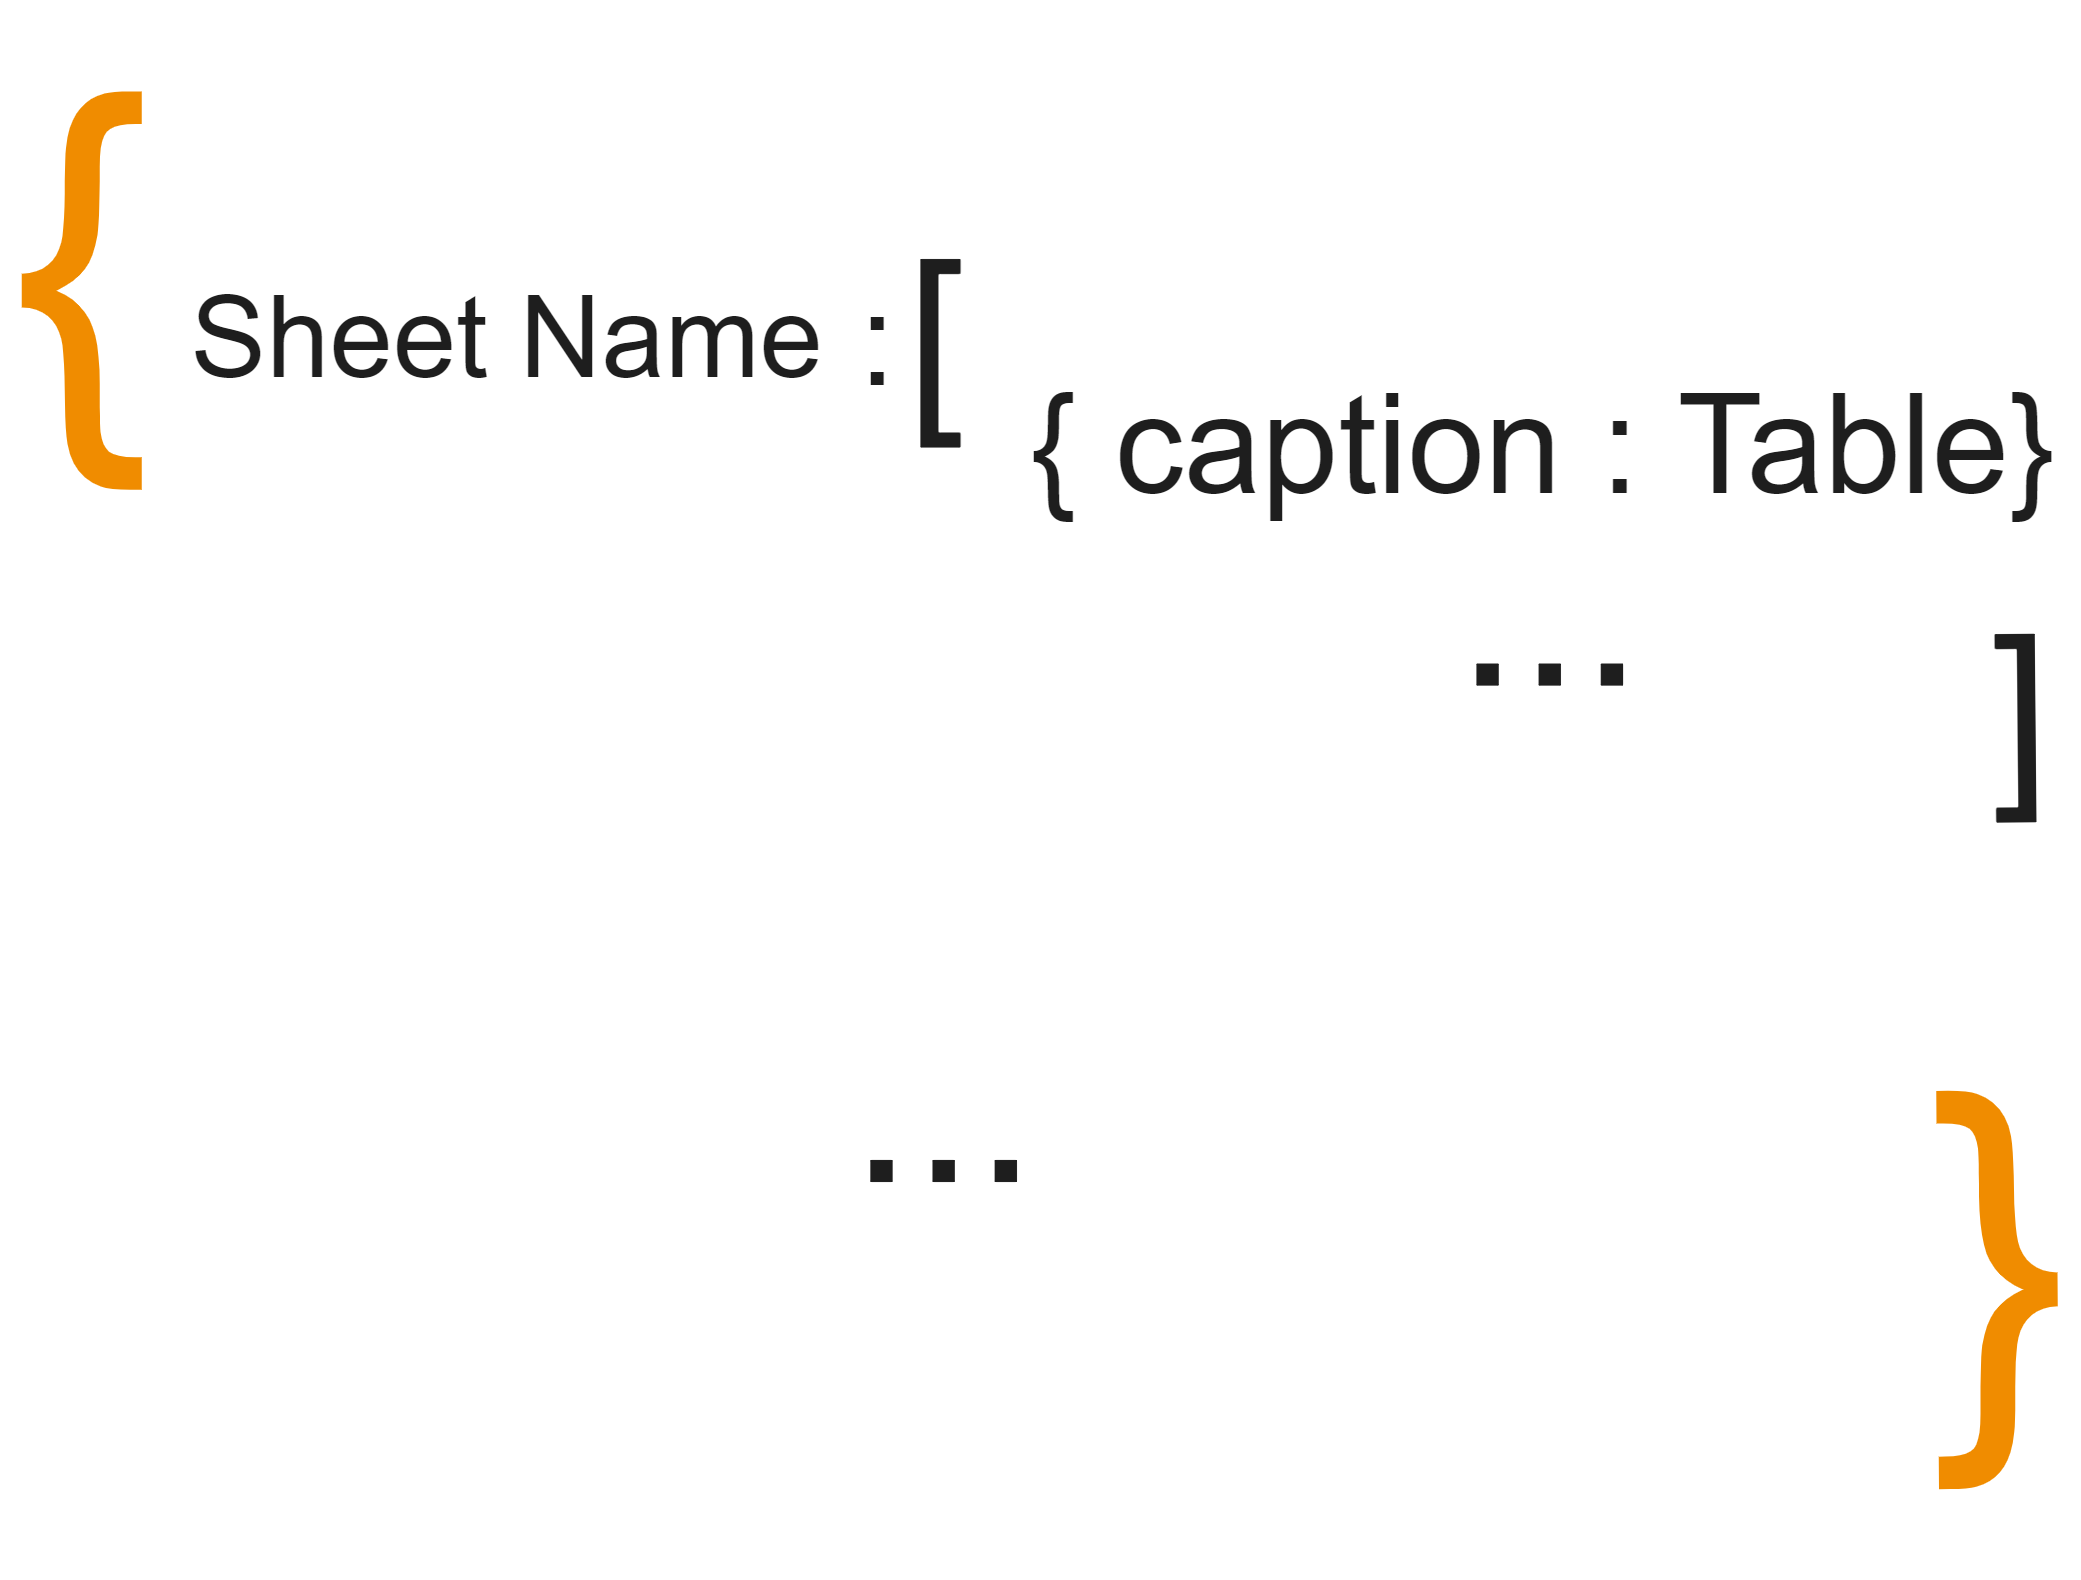
\includegraphics[width=0.4 \linewidth]{assets/organizedJson.png}
    \caption{Organized Data}
    \label{fig:org}
\end{figure}



\section{Optionnal Instructions}
In this part of the report, we talk about two cool features of our system that let users have more control over what they're working with.

\subsection{Interacting with the Order of Tables}
First, we look at how users can arrange the order of the tables. This is pretty handy because sometimes you want the tables to show up in a particular way, like having the most important one first.
\vskip 0.5cm
Imagine moving songs around in a playlist, we might have something similar as shows where you can just drag the tables into the order you like.
% \begin{figure}[H]
%     \centering
%     \includegraphics[width=0.4 \linewidth]{assets/sortCap.png}
%     \caption{Organized Data}
%     \label{fig:ord}
% \end{figure}

\subsection{Viewing Tables and Adding Instructions to Prompts}
Second, we talk about how users can see the tables right before they turn into text and add any last-minute details they think are important.

\subsubsection{Table Preview}
In our system, the capability to see tables,as shows the table, is a basic feature that enhances the user's understanding of the information being analyzed. This view only mode permits clients to see the tables as they are, without the capacity to associated specifically with the information through sorting or filtering . By showing the information in a clear, inactive format , clients can look at the structure and substance of the tables effectively . This straightforward visualization helps users assess the data more precisely and helps in planning the information for further examination or reporting . The center on a non-interactive display ensures clarity and minimizes the potential for perplexity , making it simpler for clients to interpret the information as intended.


\subsubsection{Description Generation}
Now we're getting to the really exciting part the Description Generation. This is where we take everything we've prepped and ask the language model to start making sense of it.We have our prompt ready, which is like a little message we send to the language model. This message isn't just a "hello" though; it's packed with useful stuff:
\begin{itemize}
    \item \textbf{Commands:} We include clear commands in the prompt that tell the AI exactly what to do with the table, like "Explain the trends in this sales data" or "Summarize the key findings."
    
    \item \textbf{Archive of Prior Descriptions:} If we've done this before for similar tables, we let the AI know what it said last time. It's like reminding a friend of a story they told so they don't repeat themselves.
     
    \item \textbf{Title of the Table:} Knowing the title helps the AI get the context, it's the difference between just seeing random numbers and knowing these numbers are all about, say, "Monthly Ice Cream Sales."
    
    \item \textbf{Table:} Of course, we include the table data because the AI needs to see the numbers or info it's going to talk about.
    
    \item \textbf{Custom Request Details:} And lastly, if the client threw in any extra details, like wanting to focus on a certain column or needing the description to be super simple, we put that in the prompt too.
\end{itemize}

By letting clients interact with the order of tables and see them up close , furthermore include extra instructions , we make beyond any doubt that the system does what they need . It's all around giving individuals the control to get their tables just right before they turn them into description.

\section{Document Generation}
The document generation process in our system is designed to effectively convert extracted tables from Excel into well formatted Word documents .docx , ensuring that the data presentation is both professional and accessible . This prepare is crucial for delivering significant insights in a clear and organized way . Here's how we manage each viewpoint
\subsection{Exporting Tables into a Word File}
The process of exporting tables into a Word file includes a few steps to guarantee the clarity and readability of the report:  %To begin with , we perform cell cleaning to evacuate any symbols such as '-' , indicating empty or unessential cell . Following , we consolidate cells with the same value to preserve the integrity of the tables and improve their visual appeal. Finally , we apply consistent styling and textual styles to upgrade the aesthetic presentation and guarantee that the tables are coordinates with the overall report design .
\begin{itemize}
    \item \textbf{Cell Cleaning:} As part of preparing the tables for send out, any cells containing the symbol '-', which regularly indicates empty cell or unessential information, are cleaned to seem empty. This guarantees clarity and anticipates misinterpretation of the information.
    
    \item \textbf{Merging Cells:} To preserve the integrity and readability of the tables, our system naturally combines adjacent cells that share the same value. This not only preserves the format frequently utilized in Excel to demonstrate related information but also improves the visual appeal of the table within the report format.
    
    \item \textbf{Styling and Fonts:} The aesthetic presentation of the tables is carefully managed by applying consistent styling and textual styles. This includes setting suitable textual style sizes, styles, and colors that adjust with the generally report design. This guarantees that the tables are not only readable but also visually integrated with the rest of the report.
\end{itemize}
 
\subsection{Descriptions Generation}
In our system,when creating word document, we categorize tables into two types when generating Word documents those that already have an existing description , and those that do not . For tables missing a past description , our system leverages AI to generate informative summaries for each one. This prepare involves the creation of detailed prompts that coordinate the AI to completely analyze the displayed information . The prompts are carefully crafted to emphasize important data pointsdata points and inspire particular insights from the AI. This strategy guarantees that the resulting descriptions are both exact and meaningful , providing clear and valuable summaries tailored to each table's content.

\subsection{Report Organization}
The organization of the report is essential for facilitating understanding and investigation of the information: %Each report starts with a clearly characterized title, setting the context for the consequent content . Segments are at that point utilized to organize the analysis , with each section dedicated to a particular aspect . Inside each section , tables are shown nearby their respective captions, improving the flow and coherence of the report. Also , AI generated descriptions placed below each table give valuable bits of knowledge and outlines , improving the document s utility as a comprehensive analytical tool.
\begin{itemize}
    \item \textbf{Title of the Report:} Each report starts with a clearly defined title, which sets the context for the consequent content.
    
    \item \textbf{Sections and Tables:} The report is organized into sections, each dedicated to a specific aspect of the analysis. Within each section, tables are displayed alongside their respective captions. This organizational strategy makes a difference in exploring the report and understanding the stream of data.
    
    \item \textbf{AI-Generated Descriptions:} Each table is accompanied by an AI-generated description placed immediately below the table. These descriptions serve to explain the significance of the information within the table, providing insights or summarizing patterns straightforwardly inside the report. This integration of descriptive content with financial tables improves the document's utility as a comprehensive analytical tool.
\end{itemize}

\section{Testing and Results}


\section{Limitations and Challenges}


\section{Appendices}


\section{Future Work}


\section{Conclusion}

